\section{Overview}

\subsection{Motivation}
Plasmas, commonly called the fourth state of matter, are a gas where a
significant fraction of the neutral atoms or molecules have been split into
pairs of electrons and positive ions. Initially, a curiosity of the laboratory,
they have become a critical part of every day life. The electrically charged
nature of plasmas makes them a practical means by which to convert electrical
energy into light, chemical reactions, kinetic energy, or even nuclear
reactions. From an applications perspective, they are indisposable in lighting,
semiconductor manufacturing, plastic processing, and space propulsion. On a more
broad scale, virtually all observable light in the universe is the result of a
plasma in some form or another.

Some exceptions aside, only three things are required to create a plasma: a gas,
an energy source, and a means of transferring the energy to the gas. In man-made
applications, the energy source is typically electricity, and the simplest
transfer mechanism are two electrodes placed on either side of the gas. When a
sufficient voltage is applied across the gap, residual electrons in the gas
(often created by background cosmic radiation) are accelerated until they
collide with a gas particle. The electron, having acquired a fair amount of
energy, knocks a second electron loose from the particle, leaving behind a
relatively heavy and immobile ion. Subsequently, both the first and second
electron are now accelerated by the electric field, until they again create new
electrons. Electrons continue to be created in this exponentially growing
process, referred to as an avalanche, until they cross the gap between the
electrodes, leaving behind a plasma.

Despite this relatively simple recipe, the physical characteristics can vary
greatly depending on what gas is used, what pressure it is at, what voltage is
used, whether the electricity is applied constantly or varied over time, what
kind of electrodes are used, etc. As a result, plasmas are generally produced
under tightly controlled conditions. For example, a plasma etcher used in
semiconductor manufacturing may operate at pressures that are one-thousandth of
atmospheric pressure with 99.999\% pure gases. In these plasmas, the ions and
neutral gas particles often have temperatures that are below 1,000 K. Though this
is may be above room temperature, it is well below the electrons which often
possess temperatures closer to 20,000 K. This disparity in temperatures is
characteristic of plasmas which are not in thermal equilibrium, more
colloquially known as ``low-temperature'' plasmas.

By comparison, plasmas in thermal equilibrium possess electrons, ions, and
neutral particles which are all at the same, highly elevated, temperature. For
reasons which will later be explained, such plasmas tend to occur at gas
pressures which are closer to atmosphere. High-temperature plasmas have their
own set of applications, such as arc welders which use a plasma for metal
joining. Additional examples include the xenon arc lamps used to simulate the
sun, metal-halide lamps used in cars, plasma torches for cutting metals,

Unfortunately, there are a number of applications which would benefit from
operation at higher pressures, but with low-temperatures ions and neutral
particles. This has spurred a substantial amount of research on
atmospheric-pressure plasmas (\acs{app}s) in recent years. One product of these
efforts has been the use of plasmas to treat polymers so that ink can adhere to
the surface. Another, uses low-temperature \acs{app}s to generate ozone to kill
bacterial contaminants in water.

That said, research on high-pressure, low-temperature plasmas is ongoing. The
number of potential applications has continued to grow, and the outcomes include
things like better access to clean water, wound sterilization, improved fuel
efficiency, faster airplanes, new materials, nanoparticle production, and much
more. However, these plasmas are much more difficult to create as they are
subject to a number of instabilities which either snuff out the plasma, or cause
it to transition to thermal equilibrium.

Of the few techniques available to create atmospheric plasmas, the
repetitively-pulsed nanosecond discharge (\acs{rpnd}) is unique in its ability
to create plasmas up to several liters in volume, but with relatively uniform
properties throughout. The potential of this plasma to result in even one of the
above outcomes more than warrants its close study. This is sentiment is echoed
by the National Academies, when, in their recent review of plasma science stated
that ``[high-pressure nonequilibrium plasmas] have great promise both for
practical application, and also as a unifying platform for future
low-temperature plasma science research.''

\subsection{History}

Historically, the study of low-temperature \acs{app}s has been almost
indistinguishable from the study of plasmas as a whole. However, this was not
necessarily a matter of reasoned choice. Operation at atmospheric-pressure
obviates the need for an effective vacuum pump. Additionally, prior to the
creation of large battery banks, early sources of electrical energy had
relatively small capacities. This precluded the generation of thermal plasmas
which required large amounts of energy.

Indeed, these requirements were sufficiently rudimentary that the first man-made
low-temperature \acs{app}, and plasma in general, was probably a spark generated
by rubbing fur against amber. This is commonly attributed to Thales of
Mil\^{e}tus from around 600 B.C. Electrical sparks came to intrigue many
scientists including Gottfried Liebniz, Benjamin Franklin, and Charles
Wheatstone. By the mid-1800s, Pl\"{u}cker, Gei\ss{}ler, and Hittorf began some
of the first work on low-pressure plasmas though it was Crookes who later
identified plasma as a separate state of matter. Eventually, it was J.J.\
Thomson's discovery of the electron and discretized charge that marked the
beginning of modern plasma research.

By this time, the necessary tools and techniques existed to create continuous
plasmas in pure, rarified gases. Their behavior was dominated by the motion and
interaction of the charged electrons and ions, and the presence of neutral gas
particles was undesirable. These carefully controlled systems were ideal for basic
studies of plasma behavior and were used to great effect by individuals such as
Irving Langmuir and Lewi Tonks. In fact, many modern concepts in plasma physics
can be traced back to their work.

In contrast, the pulsed \acs{app}s, characteristic of the earliest man-made
plasmas, while easy to create, were notoriously difficult to work with. Because
they did not operate in a steady state, one needed to measure how they changed
over time. This demanded a time resolution of billionths of a second.
Furthermore, such plasmas possessed large numbers of neutral particles could
confound or obscure the important behavior of the charged particles. Despite
such problems, these plasmas, including lightning, sparks, and a type that
Thomson referred to as a ``luminous front,'' retained a great deal of interest.

The culmination of these efforts was research into the so-called ``fast
ionization waves'' beginning in the 1970s and continuing to this day. These
plasmas were similar to the luminous front described by Thomson; they occurred
as an impulse of light which developed from the high voltage to the low voltage
electrode and traveled at a reasonable fraction of the speed of light. They were
generated by voltage pulses that lasted anywhere from 1-100 billionths of a
second and could reach 300 kilovolts. They could be produced in almost any gas,
and almost any pressure, provided the voltage was high enough. Furthermore,
regardless of pressure, they could uniformly fill large volumes with plasma and
highly excited neutral particles, all with little heating.

The properties of the fast ionization wave plasmas were attractive for a number
of uses, but their implementation had a number of problems. With the best
available equipment, a fast ionization wave could only be generated a few times
a second. Since the plasma quickly died away within approximately a thousandth
of a second after each pulse, this meant that a fast ionization wave plasma was
only effectively on for a percentage of the time it was operated. This had
important repercussions for plasma-processing applications where material had to
be treated as quickly as possible. Also problematic were the extremely high
voltages necessary to create these plasmas. Such voltages required complex banks
of capacitors submerged in baths of oil and careful design of the electronic
circuits and pathways to ensure reliable operation.

Recently, the invention of fast solid-state switches with low recovery times has
solved both issues. Modern switches can operate almost one-hundred thousand
times a second. This results in a plasma that is almost continually on.
Furthermore, because the plasma does not completely die away between successive
pulses, it requires much lower voltages to reignite with each pulse. Where
before the fast ionization wave may have been prohibitively large and expensive
for a number of situations, the repetitively-pulsed nanosecond discharge is able
to serve as a more capable substitute.

\subsection{Questions}

The large pedigree of pulsed plasma research belies the fact that they are not
well-understood. The short time scales, electrical noise, high pressures, and
complex chemistries continue to stymie the best experimental equipment and most
well-developed simulations. This is particularly true of \acs{rpnd}s which have
recently emerged as an area of interest. These discharges present a number of
questions with a range of implications in their use and development.

Most fundamentally, the majority of \acs{rpnd} research has concentrated on
quantities which do not change over time, or change slowly compared to the
formation time. The most common of these are chemical composition, gas
temperature, total energy deposited. While undoubtedly important, such
measurements provide little insight on what is happening while the plasma is
forming. Thus the question arises, what are the plasma properties during its
formation?

Additionally, the most of the contemporary studies have focused on system in
mixtures of molecular gases such as oxygen, nitrogen, air, and occasionally
hydrogen. The choice of these gases reflect a limited number of specific
applications. However, several others involve the use of rare gases, such as
helium. Notably, rare gas atoms feature unique internal structures which can
significantly influence the properties of a plasma. So we naturally would like
to address how a rare gas \acs{rpnd} compares one in a molecular gas.

Finally, the persistence of the plasma between pulses can alter the development
of the discharge. For example, a large background population of electrons can
quickly shield out the applied voltage pulse. This would have the
counterintuitive effect of decreasing the final electron density despite a large
number of seed electrons. As a result, it is important to study how the trends
of various parameters and how they're optimized for different conditions. This
is particularly important for application purposes where some excited states are
more desirable than others.

\subsection{Approach}

In order to answer these questions, I present a series of experiments,
measurements, and simulations of a helium \acs{rpnd}.

Here, I present a series of experiments, measurements, and simulations used to
study the dynamics of a helium \acs{rpnd}. Helium was chosen because it is
commonly used in gas mixtures to stabilize the plasma between pulses, in
addition, it provides a relatively simple atomic system for which a wealth of
the necessary electronic, optical, and atomic data are available.




Here, I present the results of a study into the dynamics of a \acs{rpnd}. The
primary experimental measurements are laser-absorption spectroscopy of the
helium metastable level, supported by calibrated optical emission measurements.
The measurements are interpreted with the aid of a helium global model and
particle-in-cell simulations.

\section{Literature Review}

\acs{rpnd}s are only a recent invention which resulted from advances in
fast-switching semiconductors. However, the physics of their formation is
related to a much larger category of plasmas which includes lightning, sparks,
and even some transient phenomena in DC glows. These plasmas are unique in that
their formation occurs on timescales much faster than the traditional Townsend
mechanism allows for. The means by which these plasmas form has acquired several
names in the literature; here we will adopt the term, fast ionization wave
(\acs{fiw}).\footnote{It should be noted that the phrase wave does not indicate
any kind of periodic motion or spatial arrangement. Simply put, it describes a
boundary which separates ionized and unionized gas which travels from one
electrode to another.}.

\subsection{Early History of Pulsed Discharges}

The first \acs{fiw} was likely generated by Wheatstone in 1835
\cite{Wheatstone1835}. As reported by Thomson \cite{Thomson1893}, Wheatstone
built a vacuum tube six feet in length, and applied a high voltage across the
gas. As a plasma formed in the tube, Wheatstone observed its formation with a
rotating mirror. The use of this apparatus allowed Wheatstone to place a lower
limit on the speed with which the plasma travelled from one electrode to the
other. Though the discharge crossed the tube with a speed of at least
$8\times10^7$ cm/s, spectral observations indicated that the particles emitting
the light were not travelling at that speed \cite{Zahn1879}.

Later, Thomson revisited this work with an improved apparatus
\cite{Thomson1893}. This included a tube that was now 15 m in length and five mm
in diameter, as seen in figure \ref{fig:thomson}.
\begin{figure}
  \centering
  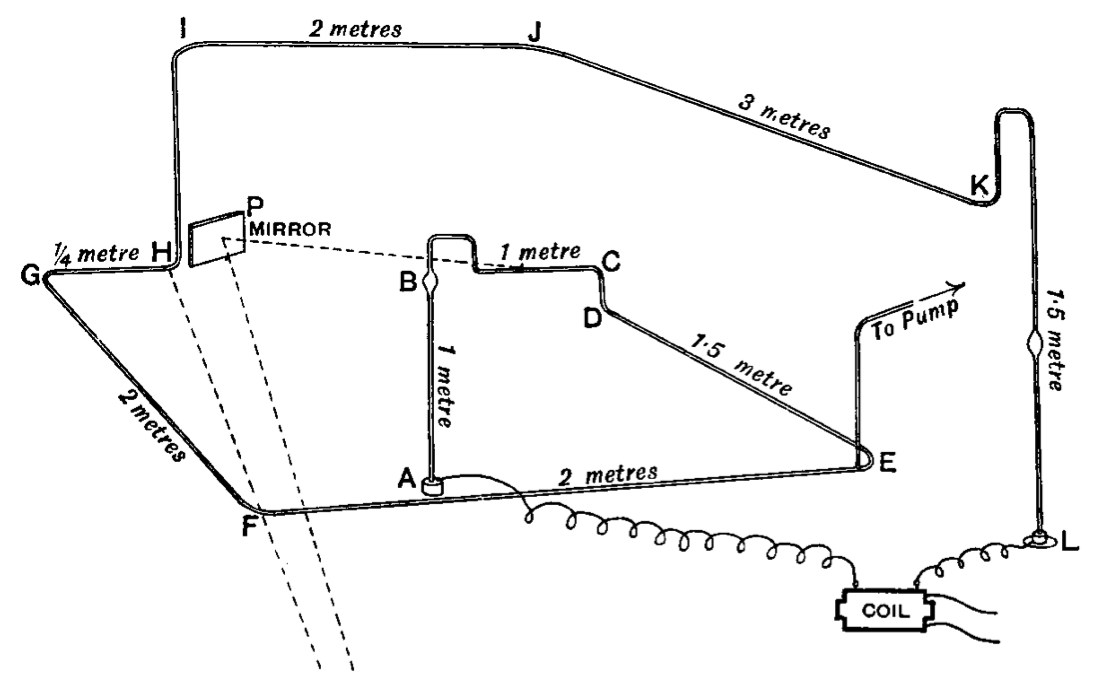
\includegraphics[width=4in]{chapters/introduction/figures/thomson.png}
  \caption{A sketch of J.J. Thomson's early experiments on fast ionization
  waves in long vacuum tubes.}\label{fig:thomson}
\end{figure}
Also using the rotating mirror apparatus, Thomson was able to greatly improve on
the estimates of Wheatstone. He estimated that the so-called ``luminous front''
had a speed that was more than $1.5\times10^{10}$, or in excess of half of the
speed of light. Furthermore, Thomson determined that the front always appeared
to travel from the positively pulsed electrode (anode) to the ground electrode
(cathode).

The study of these luminous fronts was revisited by several researchers in the
wake of Thomson \cite{James1904, Whiddington1925, Beams1926} with varied
success. By his own admission, Beams's work in 1926 was done ``hurriedly,''
using a rudimentary Kerr cell. In 1930, Beams returned to the propagation of
light pulses in vacuum tubes with a rotating mirror apparatus \cite{Beams1930}.
In addition to confirming his previous measurements, and those of Thomson, Beams
discovered that the \acs{fiw} always traveled from the electrode with the
highest absolute potential, to the lowest one. In other words, the wave could be
anode or cathode directed, depending on the magnitude of their potentials
relative to ground. Benefiting from an improved understanding of electricity,
namely the existence of electrons and ions, Beams was able to provide the first
hypothesis on the nature of the \acs{fiw}:
\begin{quote}
  In the neighborhood of the electrode $\ldots{}$ the field is very high and
  intense ionization should take place. This ionization due to the large
  difference in mobilities of positive ions, negative ions and electrons
  respectively should result in the establishment of a space charge. This space
  charge, once formed near the high potential electrode $Q$ must move down the
  tube regardless of the polarity of the applied potential because of the
  changes it produces in the field near its edges.
\end{quote}

At about the same time, Schonland and Collens reported on their observations of
lightning \cite{Schonland1933}. Though the general structure and length scale of
lightning is substantially different from the luminous fronts observed by Beams
and Thomson, the two phenomena would later prove to be very similar. In their
work Schonland and Collens noted that lightning would usually occur in a
two-step process. Based on the images they obtained, they suggested that
the leader was generated by a relatively small ``dart'' with a mean vertical
velocity of $7.2\times10^8$ cm/s. The dart moved in a random manner, changing
directions at random intervals, but always moving downward.

The second step began when this dart reached the ground. Once there, a bright
return stroke would occur along the same path that the leader had traced out. In
contrast to the leader stroke, the return stroke had a velocity of $5\times10^9$
cm/s. Schonland and Collens hesitantly attributed the leader stroke to an
extended electron avalanche, and the return stroke to thermal ionization along
the conductive path generated by the dart. However, calculations by Cravath and
Loeb showed that the speeds of the proposed avalanche would have to be
inconsistent with the fields at the head of a lightning stroke
\cite{Cravath1935}. Instead, they suggested that the dart was actually a moving
region of space charge which locally accelerated electrons to ionizing energies.
This was fundamentally similar to the mechanism proposed by Beams in 1930.

\subsection{The Streamer Model}

It was long known that sparks in air were similar to lightning. Advances in
technology during the 1930's led to experiments which reinforced this
similarity. In response to the measurements of Schonland and Collens; Snoddy,
Beams, and Dietrich studied the breakdown of gas in a long tube with an
oscillograph \cite{Snoddy1936}. The results from the oscillograph showed a very
clear return wave for which they measured several parameters the characterized
as a function of pressure and applied potential. They observed that at low
voltages, the system behaved like a large resistor in series with a capacitor,
and below a critical voltage, no return stroke would form. Finally, in order to
explain the propagation of the \acs{fiw} generated by the positive pulse, they
suggested that photoionization was occurring in the space ahead of the wave.

Around the same time, Flegler and Raether had come to a similar conclusion,
leading to the first attempt at a theory describing streamers
\cite{Flegler1936}. This same theory was proposed independently by Loeb and Meek
in a series of papers \cite{Loeb1940, Loeb1940a, Meek1940}. The streamer theory
divided the initial breakdown of a spark into two steps. In the first step, an
electron avalanche is initiated between two electrodes. The avalanche travels
toward the anode and leaves behind a region of high positive space charge. In
the second step, the return stroke begins at the cathode and travels toward the
cathode. It was suggested that the head of the return stroke ionizes the gas
ahead of it by pulling in background electrons or via photoionization.
\footnote{These early works emphasized the importance of photoionization. It is
now know that it is only required for cathode-directed streamers in systems with
no background ionization. In addition, Mesyats later showed that the lifetime of
the excited states responsible for photoionization were often longer than the
lifetime of the streamers \cite{Mesyats1972}}.

The streamer model proved relatively successful in describing the development of
sparks and lightning. Theoretical estimates of the speed matched the velocity
measurements that were acquired through photographs and oscillographs.
Additionally, the theory is able to account for the halting manner in which
lightning is formed, though it is only tentatively able to describe the
branching and stepped appearance. Finally, the streamer mechanism provides an
adequate explanation of why streamer discharges are not affected by the shape or
material of the cathode, namely, they do not depend on secondary electron
emission.

The study of the formation of streamers and lightning continues to be active to
this day. Following the initial work of Flegler, Raether, Loeb, and Meek, a
number of researchers began to explore the boundary between the Townsend
mechanism and the streamer mechanism. Most notable was Fisher and Bederson's
work in 1951 \cite{Fisher1951}, which was later extended to nitrogen
\cite{Kachickas1952} and argon \cite{Kachickas1953}. However, there were still a
number of phenomena that were poorly explained by the streamer model. In
particular, Kunhardt provided a useful overview of the problems in 1980
\cite{Kunhardt1980}. However, even before that, it was apparent that the
transients of sparks and lightning was more complicated than thought.

\subsection{Ionizing Waves of Potential Gradient}

Per Chalmers \cite{Chalmers1971}, Rogowski and Buss \cite{Rogowski1927,
Buss1932} observed a fast, diffuse, glow discharge immediately prior to the
filaments which often accompany a streamer discharge. Allibone and Meek, noted
similar diffuse discharges in air based on oscillographs and photographs
\cite{Allibone1938, Allibone1938b, Allibone1938c}. However, the Boys apparatus
which was employed in these studies (an ancestor to the modern streak camera)
was unable to capture the evolution of the diffuse glow, given its large spatial
extent.

This was first noted by Allibone who attempted to use Lichtenberg
figures\footnote{Such figures directly exposed photographic emulsions to the
electrical discharge. The developed image was a time-integrated representation
of the discharge.} to definitively capture this diffuse glow
\cite{Allibone1948}. Later, Saxe and Meek used the recently invented
photomultiplier tube to record the evolution of the light emissions in the
brief, diffuse glow \cite{Saxe1948} as a function of space. Both studies
agreed in the existence of the diffuse glow, despite some disagreement on the
nature of its geometry and propagation.

The similarity of fast, transient, ionization waves in certain glow discharges
\cite{Westberg1959} to the development of lightning and streamers led Loeb to to
the conclusion that they were all the same phenomena \cite{Loeb1965}. He 
referred to them as ``ionizing waves of potential gradient.'' Loeb stated that
such waves required the generation of a steep potential gradient in a
sufficiently short period of time.

As reported by Babich, Loika, and Tarasova \cite{Babich1977}, the detection of
x-ray emissions from pulsed, high-pressure, helium discharges created a new
avenue of interest for these transient plasmas \cite{Stankevich1967,
Noggle1968}. Unlike the streamers, which were often filamentary, these new
discharges exhibited surprising uniformity. The primary difference being the
duration of the pulse (on the order of nanoseconds) and the applied potentials
(in excess of 200 kV).

The x-rays suggested that electrons in these discharges were accelerated to
unusually high energies (on the order of 10 keV) despite the high collisionality
implied by the high gas pressures. This prompted Babich and Stankevich to
suggest that the x-rays resulted from continually accelerated electrons
impinging on the metal electrodes \cite{Babich1973}. Briefly, the electric
fields in the fronts of the ionizing waves were so large that they managed to
accelerate electrons well past the peak in their collisional cross sections.

The presence of runaway electrons was sufficient to explain the production of
x-rays, however it did not sufficiently address the uniformity of these
discharges. After several experiments, Mesyats, Bychov, and Kremnev came to the
conclusion that these transient plasmas were the result of many simultaneous
avalanches occurring throughout the gas volume. This contrasts with the
classical view of the streamer which involves only a single avalanche. Kunhardt
and Byszewski later expanded on this work by developing a kinetic model to
explain the behavior of all pulsed discharges above the Townsend threshold
\cite{Kunhardt1980}.

It was based on the studies of the fast electrons in these discharges that
Mesyats, Bychov, and Kremnev proposed the use of a fast electron beam for
pumping high-pressure gas lasers. Similar work was conducted simultaneously by
Fenstermacher et al.~\cite{Fenstermacher1972}. Later, Hunter \cite{Hunter1976},
and Koval'chuk and Mesyats \cite{Koval'chuk1976} proposed that such discharges
be used for fast-closing switches. The need for a homogeneous plasmas in these
applications prompted Palmer \cite{Palmer1974}, and Levatter and Lin
\cite{Levatter1980} to investigate the necessary conditions for uniformity. They
concluded that the primary requirement for uniformity was a threshold value of
fractional ionization.

\subsection{Repetitively-Pulsed Nanosecond Discharges}

The type of discharge originally studied by Babich, Loika, and Tarasova came to
be known as the fast ionization wave (\acs{fiw}). In the years following its
discovery, a substantial effort was made to document the properties of the
\acs{fiw} over a wide range of conditions. In these studies, the wave velocity,
current, and attenuation were the most frequently measured quantities. Much of
this work is summarized in a review by Vasilyak \cite{Vasilyak1994}. Also
reviewed are Slavin and Sopin's work which was the first to attempt a
computation of the electron energy distribution function \acs{eedf} in
\acs{fiw}s \cite{Slavin1992}.

The experimental measurements and computational work reported by Vasilyak were
expanded on by studies conducted at the Moscow Institute of Physics. These are
reviewed by Starikovskaia et al.~\cite{Starikovskaia2001} and included
measurements of the electron density, electric field, and energy coupling for
\acs{fiw}s in air, nitrogen, and hydrogen. The work by Starikoskaia and
Starikovskii still represent the most detailed study of the \acs{eedf}
in \acs{fiw}s, however its focus was limited to negative discharges in nitrogen.

However, Starikovskaia et al. noted that the usefulness of \acs{fiw}s was
limited by their repetition rates. The power supplies for \acs{fiw}s were
capacitor banks, charged in parallel, and discharged in series (also referred to
as the Marx bank). Unfortunately, the spark gaps used to trigger these
capacitor banks would not operate above a few hundred Hz. This changed in the
late 1990's with the development and commercialization of fast, solid-state
switches. Specifically, the fast ionization dynistor allowed repetition rates of
100 kHz.

This led to a new class of repetitively-pulsed discharges, or the \acs{rpnd}.
These discharges were operated at sufficiently high rates such that charged
particles would persist between pulses. Not only did this increase the effective
on-time of the plasma, but this residual ionization made it much easier to
obtain a stable discharge with lower voltages. This reflects the preionization
threshold that was earlier identified by Levatter and Lin.

The improved qualities of the \acs{rpnd} over the \acs{fiw} inspired a number of
application-driven studies. This included:
\begin{itemize}
  \item Plasma-assisted combustion \cite{Pancheshnyi2006, Starikovskaia2006, 
        Adamovich2008}
  \item Magnetohydrodynamic energy bypass engines \cite{Macheret2002,
        Adamovich2008, Schneider2009a}
  \item Plasma actuators \cite{Starikovskii2009, Adamovich2009}
  \item High-pressure xenon lamps \cite{Nikandrov2008}
  \item Plasma medicine \cite{Ayan2009, Zimmerman2012}
  \item Water treatment \cite{Foster2013}
\end{itemize}
Though not specific to the \acs{rpnd}, Becker et al. \cite{Becker2005} provide
an extensive discussion of the potential uses for non-equilibrium air plasmas.

As a result, contemporary researchers have produced a wealth of literature on
the operation of \acs{rpnd}s. More recently, there have been detailed
measurements of the gas temperatures \cite{Pilla2006, Pancheshnyi2006,
Nishihara2006, Bao2007, Lou2007, Pai2009, Zuzeek2010, Nishihara2011}, chemical
composition \cite{Bao2007, Lou2007, Pai2009}, electric fields \cite{Ito2009,
Ito2010, Muller2011a}, and energy coupling \cite{Macheret2006, Pancheshnyi2006}.
Notably, these studies have been generally restricted to molecular gases; air,
nitrogen, and occasionally, hydrogen.

The first such study was the work of Laroussi and Lu who examined a
\acs{rpnd} excited in a stream of helium flowing from a tube into air
\cite{Laroussi2005, Lu2006}. The resulting plasma had the appearance of a jet,
emitted from the open end of the tube. Using fast photography they observed that
the jet was actually a series of plasma ``bullets'' formed with each pulse.
Measurements of the bullet velocities showed that their speed greatly exceed
what would be expected purely from electrons drifting under the applied electric
field. They concluded that the bullets were essentially cathode-directed
streamers which propagated with the aid of photoionization.

The work of Laroussi and Lu spawned a great deal of interest in \acs{rpnd}
helium plasma jets\footnote{A distinction should be made between plasma jets,
excited by sinusoidal power supplies, similar to the well-known
dielectric-barrier discharge \cite{Kogelschatz2003}, and those produced by
nanosecond pulses. Differences between the two were reported by Walsh, Shi, and
Kong \cite{Walsh2006}.} For example, Walsh et al. studied the atomic oxygen
production for helium-oxygen mixtures with the use of emission spectroscopy and
a global plasma chemistry model \cite{Walsh2010}. Urabe et al. employed a
variety of laser diagnostics to measure the radial density profiles of helium
metastable atoms and molecular nitrogen ions in a similar jet. This work was
supported by a number of two-dimensional plasma simulations such as those by
Naidis \cite{Naidis2010} and Breden, Miki, and Raja \cite{Breden2011}.

Simultaneously, study of large-volume \acs{rpnd}s has received little attention
even as the study of single fast ionization waves has declined. The recent work
by Takashima et al. represents one of the most complete studies of a \acs{fiw},
featuring two-dimensional fluid simulations, an analytic model, and capacitive
probe measurements in helium and nitrogen \cite{Takashima2011}. For the measured
parameters, the experimental and numerical results showed good agreement.

However, there is reason to believe that a \acs{rpnd} in a similar geometry
would exhibit different characteristics. The authors note that changes in the
initial electron density can cause significant changes in the peak electric
field, final electron density, and wave velocity. Furthermore, little effort has
been made to study the excited state dynamics of rare gas \acs{fiw}s or
\acs{rpnd}s. However, some of these excited states can play an important role as
long-lived electron sources \cite{Nersisyan2004}, and as a source of anomalous
electron heating \cite{Wells1973}. Finally, measurements of excited state
densities can provide important benchmarks for computational simulations.
